\documentclass[12pt,a4paper]{article}
\usepackage[utf8]{inputenc} %polskie znaki
\usepackage[T1]{fontenc}	%polskie znaki
\usepackage{amsmath}		%matematyczne znaczki :3
\usepackage{enumerate}		%Dodatkowe opcje do funkcji enumerate
\usepackage{geometry} 		%Ustawianie marginesow
\usepackage{graphicx}		%Grafika
\usepackage{wrapfig}		%Grafika obok textu
\usepackage{float}			%Allows H in fugire
\pagestyle{empty} 			%usuwa nr strony

\newgeometry{tmargin=2cm, bmargin=2cm, lmargin=2cm, rmargin=2cm} 

\begin{document}
		\begin{center}
		\LARGE Planimetria
	\end{center}
	\vspace{1.5cm}
	\begin{enumerate}[1.]
		
		\item Oblicz brakujące boki trójkątów
				
		\begin{figure}[h]
			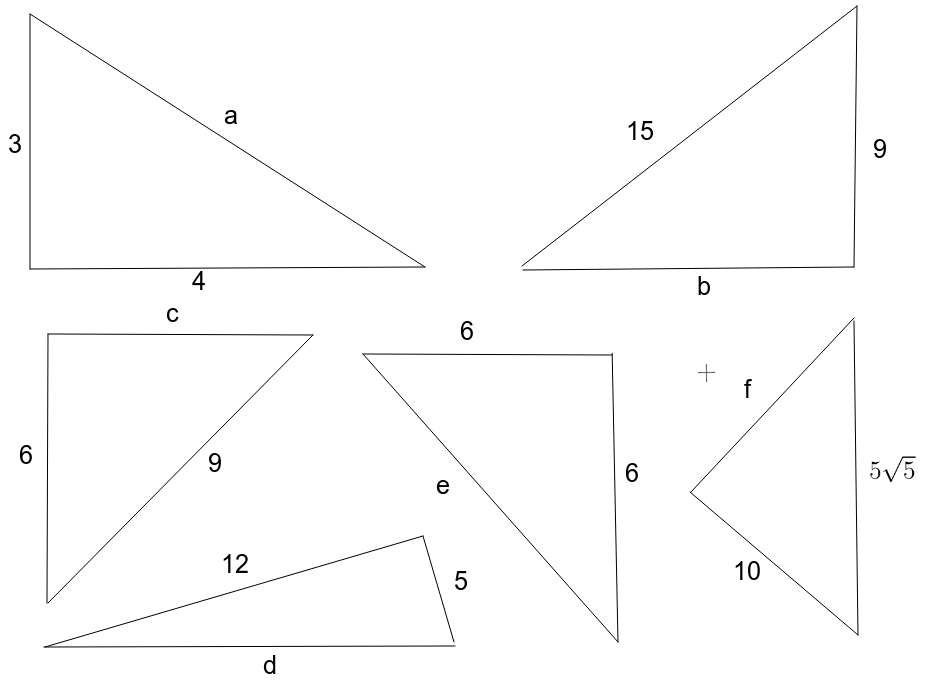
\includegraphics[scale=0.7]{plan2}
		\end{figure}
		
		\item Boki prostokąta mają długości $6-\sqrt{13}$ i $6+\sqrt{13}$. Oblicz długość przekątnej tego prostokąta.
		
		\item Przekątna prostokąta ma długość $5\sqrt{5}$, a jeden z jego boków jest dwa razy dłuższy od drugiego. Oblicz pole tego prostokąta.
		
		\item Przyprostokątne pewnego trójkąta prostokątnego mają długości 12 i 16. Oblicz wysokość obliczoną na przeciwprostokątną.
		
		\newpage
				
		\item Oblicz miary kątów $\alpha$ i $\beta$, gdzie:
	
		\begin{enumerate}[a)] \begin{tabular}{p{7cm} p{7cm}}
				\item odcinek $CD$ to wysokość & \item odcinek $CD$ to dwusieczna \\
		\end{tabular} \end{enumerate}
		
		\begin{figure}[h]
			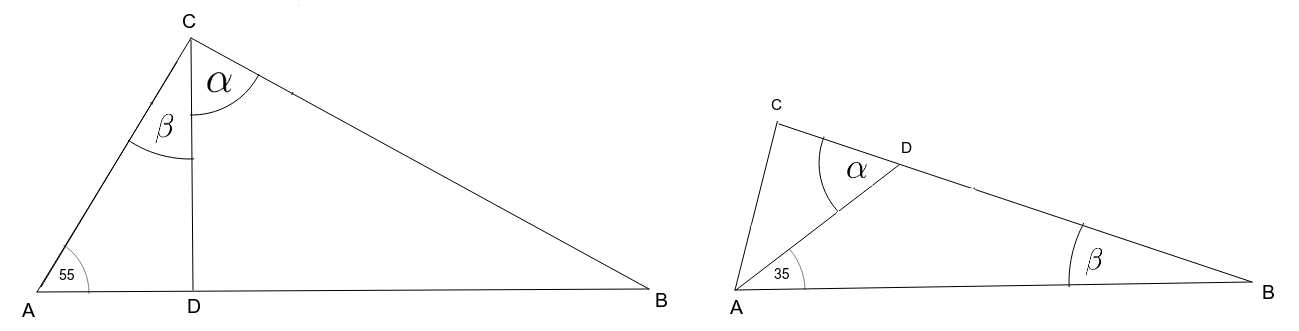
\includegraphics[scale=0.5]{plan1}
		\end{figure}
	
		\item Przeciwprostokątna w trójkącie prostokątnym wynosi 12cm. Środkowe trójkąta przecinają się w punkcie P. Oblicz długość środkowej opuszczonej na przeciwprostokątną oraz długości odcinków, na które punkt P dzieli środkową.
		
		\item W trójkącie $ABC$ środkowa opuszczona z wierzchołka $C$ jest dwa razy krótsza od boku $AB$. Wyznacz miarę kąta $ABC$.
		
		\item Środkowe w trójkącie równoramiennym mają długości 12, 12 i 3. Oblicz długości boków tego trójkąta. (Podopowiedź: Środkowe przecinają się w stosunku 2:1)
		
		\item W trójkącie równoramiennym ramię jest dwa razy dłuższe od wysokości opuszczonej na podstawę. Oblicz pole trójkąta, jeśli podstawa ma długość 12.
		
		\item Długość podstawy trójkąta równoramiennego wynosi $4\sqrt{5}$, a wysokość opuszczona na tę podstawę jest równa 4. Oblicz długość ramienia trójkąta oraz wysokość opuszczoną na ramię trójkąta.
		
		\item Oblicz pole trapezu
		
		\begin{figure}[h]
			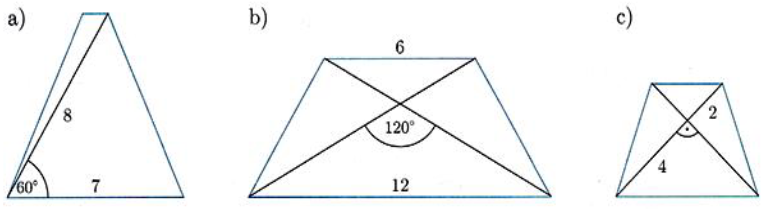
\includegraphics[scale=0.8]{plan3}
		\end{figure}
		\newpage
		\item Wyznacz miary kątów $\alpha$, $\beta$
		
		\begin{figure}[h]
			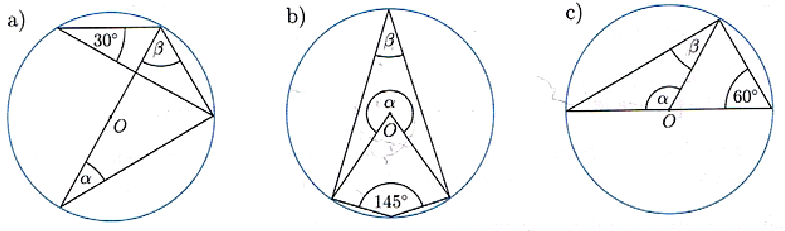
\includegraphics[scale=0.8]{plan4}
		\end{figure}
	
		\item Wyznacz miarę kąta $\alpha$
		
		\begin{figure}[h]
			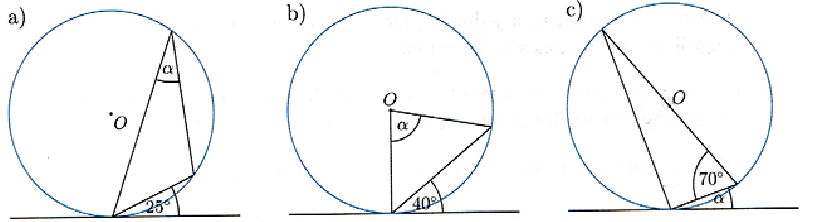
\includegraphics[scale=0.8]{plan5}
		\end{figure}
		
		\item Promień okręgu opisanego na trójkącie równobocznym jest równy 8. Oblicz wysokość tego trójkąta.
		
		\item Na trójkącie prostokątnym, którego przyprostokątne mają długości 12 i 9 opisano okrąg. Oblicz promień tego okręgu.
		
		\item Na trójkącie równobocznym opisano okrąg o długości $4\pi$. Oblicz długość boku tego trójkąta.
		
		\item Oblicz długość promienia okręgu opisanego na trójkącie równoramiennym o bokach 4, 6 i 6.
		
		\item Oblicz promień okręgu opisanego na trójkącie prostokątnym o przyprostokątnych długości 1 i 7.
		
		\item Kwadrat, którego obwód wynosi 8, wpisano okrąg i opisano okrąg. Oblicz różnice pól tych okręgów.
		
		\item Pole powierzchni trójkąta jest równe 6, a długość promienia okręgu wpisanego w ten trójkąt wynosi 3. Oblicz obwód tego trójkąta.
		
		\item Oblicz pole okręgu wpisanego w kwadrat o przekątnej długości 6.
		
	\end{enumerate}
\end{document}